\documentclass[11pt,t,usepdftitle=false,aspectratio=169,usenames,dvipsnames]{beamer}
\usetheme[nototalframenumber,foot,logo]{uibk}
\headerimage{3}

\usepackage[T1]{fontenc}
\usepackage{xcolor}
\usepackage{minted}
\usepackage{tikz}
\usetikzlibrary{calc}

\title{Making CoAP.NET great again!}
\subtitle{Is it worth to await?}
\author{Philip Wille}

\begin{document}
    \maketitle{}

    \begin{frame}
        \frametitle{Introduction}
        \begin{itemize}
            \item<1-> Synchronous and asynchronous execution
            \item<2-> \textbf{T}ask-based \textbf{A}synchronous \textbf{P}attern (TAP)
            \item<3-> \textbf{Co}nstrained \textbf{A}pplication \textbf{P}rotocol (CoAP)
        \end{itemize}
    \end{frame}

    \begin{frame}
        \frametitle{Write synchronous code in C\#}
        \inputminted[framesep=2mm, baselinestretch=1.2, funcnamehighlighting=true, fontsize=\footnotesize, linenos]{csharp}{codes/example_synchronous.cs}
    \end{frame}

    \begin{frame}
        \frametitle{Synchronous execution}
        \begin{figure}[ht]
            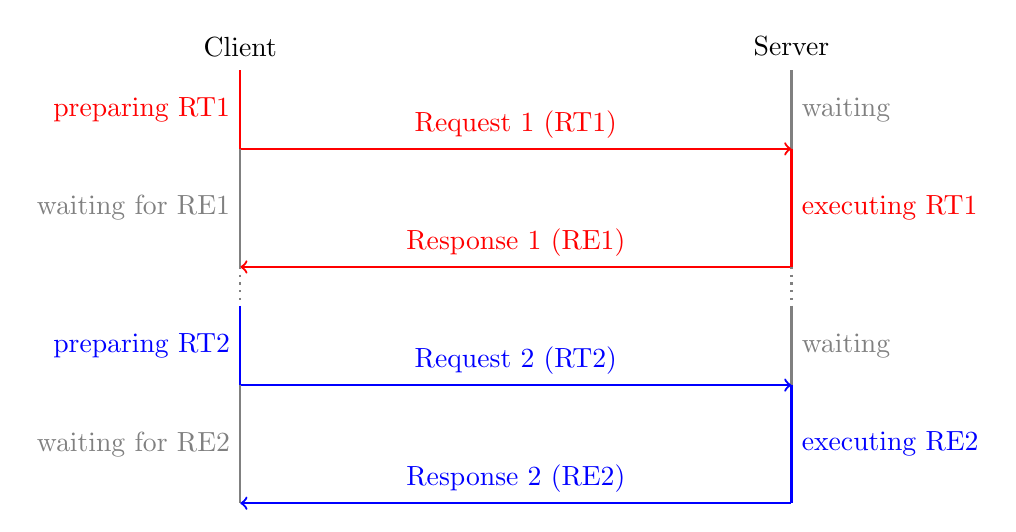
\begin{tikzpicture}
                \node at (-3,.3) {Client};
                \node at (4,.3) {Server};

                \draw[thick, red] (-3,0) -- node[left] {preparing RT1}(-3,-1);
                \draw[thick, gray] (4,0) -- node[right] {waiting} (4,-1);
                \onslide<1->
                \draw[->, thick, red] (-3,-1) -- node[midway,above] {Request 1 (RT1)} (4,-1);
                \onslide<2->
                \draw[thick, gray] (-3,-1) -- node[left] {waiting for RE1} (-3,-2.5);
                \draw[thick, red] (4,-1) -- node[right] {executing RT1} (4,-2.5);
                \onslide<3->
                \draw[<-, thick, red] (-3,-2.5) -- node[midway,above] {Response 1 (RE1)} (4,-2.5);
                \onslide<4->
                \draw[dotted, thick, gray] (-3, -2.5) -- (-3, -3);
                \draw[dotted, thick, gray] (4, -2.5) -- (4, -3);
                \onslide<5->
                \draw[thick, blue] (-3,-3) -- node[left] {preparing RT2}(-3,-4);
                \draw[thick, gray] (4,-3) -- node[right] {waiting} (4,-4);
                \onslide<6->
                \draw[->, thick, blue] (-3,-4) -- node[midway,above] {Request 2 (RT2)} (4,-4);
                \onslide<7->
                \draw[thick, gray] (-3,-4) -- node[left] {waiting for RE2} (-3,-5.5);
                \draw[thick, blue] (4,-4) -- node[right] {executing RE2} (4,-5.5);
                \onslide<8->                
                \draw[<-, thick, blue] (-3,-5.5) -- node[midway,above] {Response 2 (RE2)} (4,-5.5);
            \end{tikzpicture}
        \end{figure}
    \end{frame}

    \begin{frame}
        \frametitle{Asynchronous execution}
        \begin{figure}[ht]
            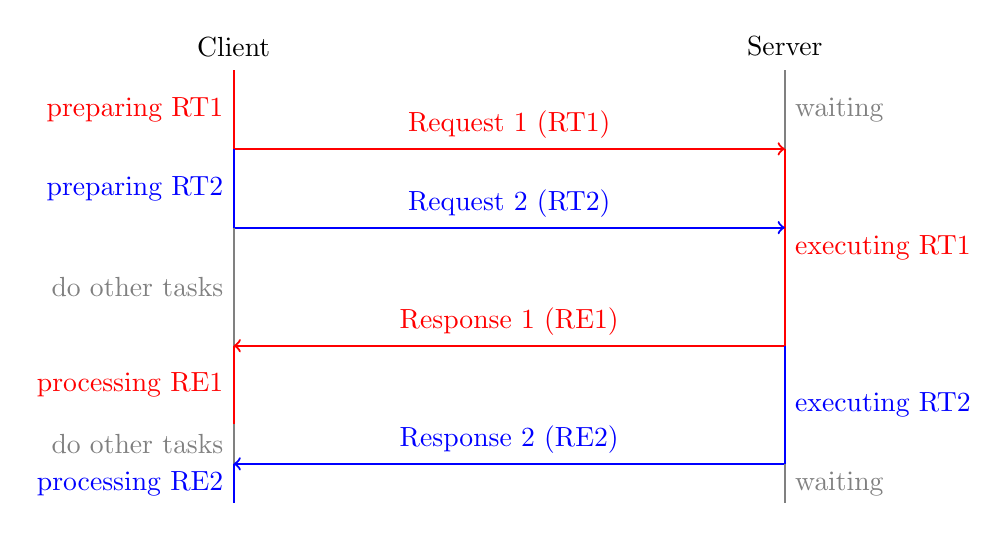
\begin{tikzpicture}
                \node at (-3,.3) {Client};
                \node at (4,.3) {Server};

                \draw[thick, red] (-3,0) -- node[left] {preparing RT1}(-3,-1);
                \draw[thick, gray] (4,0) -- node[right] {waiting} (4,-1);
                \onslide<1->
                \draw[->, thick, red] (-3,-1) -- node[midway,above] {Request 1 (RT1)} (4,-1);
                \onslide<2->
                \draw[thick, red] (4,-1) -- node[right] {executing RT1} (4,-3.5);
                \onslide<3->
                \draw[thick, blue] (-3,-1) -- node[left] {preparing RT2} (-3,-2);
                \onslide<4->
                \draw[->, thick, blue] (-3,-2) -- node[midway,above] {Request 2 (RT2)} (4,-2);
                \onslide<5->
                \draw[thick, gray] (-3,-2) -- node[left] {do other tasks} (-3,-3.5);
                \onslide<6->
                \draw[<-, thick, red] (-3,-3.5) -- node[midway,above] {Response 1 (RE1)} (4,-3.5);
                \onslide<7->
                \draw[thick, blue] (4,-3.5) -- node[right] {executing RT2} (4,-5);
                \onslide<8->
                \draw[thick, red] (-3,-3.5) -- node[left] {processing RE1}(-3,-4.5);
                \onslide<9->
                \draw[thick, gray] (-3,-4.5) -- node[left] {do other tasks} (-3,-5);
                \onslide<10->
                \draw[<-, thick, blue] (-3,-5) -- node[midway,above] {Response 2 (RE2)} (4,-5);
                \onslide<11->
                \draw[thick, blue] (-3,-5) -- node[left] {processing RE2} (-3,-5.5);
                \draw[thick, gray] (4,-5) -- node[right] {waiting} (4,-5.5);
            \end{tikzpicture}
        \end{figure}
    \end{frame}

    \begin{frame}
        \frametitle{Write asynchronous code in C\#}
        \inputminted[framesep=2mm, baselinestretch=1.2, funcnamehighlighting=true, fontsize=\footnotesize, linenos]{csharp}{codes/example_asynchronous.cs}
    \end{frame}
\end{document}